\documentclass[12pt, letterpaper]{article}
\usepackage{graphicx} % Required for inserting images
\graphicspath{{./figures/}}
\usepackage{listings} % Required for inserting code
\lstset{inputpath=./src/}
\usepackage{xcolor} % Required for formatting code

\title{Assignment 2 - LaTeX Write Up}
\author{Connor Fleischman}
\date{November 1, 2024}

\definecolor{background}{rgb}{0.95,0.95,0.92}
\definecolor{codegreen}{rgb}{0,0.6,0}
\definecolor{codegray}{rgb}{0.5,0.5,0.5}
\definecolor{codepurple}{rgb}{0.58,0,0.82}
\definecolor{magenta}{rgb}{1,0,1}
\definecolor{backcolour}{rgb}{0.95,0.95,0.92}
\definecolor{keywordcolor}{rgb}{0.82,0.1,0.26}

\lstdefinestyle{mystyle}{
   backgroundcolor=\color{background},   
   commentstyle=\color{codegreen},
   keywordstyle=\color{keywordcolor}\bfseries,
   numberstyle=\tiny\color{codegray},
   stringstyle=\color{codepurple},
   basicstyle=\ttfamily\small,
   frame=single, 
   rulecolor=\color{codegray},
   breakatwhitespace=false,         
   breaklines=true,                 
   captionpos=b,                    
   keepspaces=true,                 
   numbers=left,                    
   numbersep=10pt, 
   showspaces=false,                
   showstringspaces=false,
   showtabs=false,                  
   tabsize=4,
   emph={int,char,double,float,unsigned}, 
   emphstyle={\color{blue}},
}

\lstset{style=mystyle}

\begin{document}
\maketitle

\section{Assignment Results} \label{AssignmentResult}
Assignment 02 was to perform different searches on the magic items text file provided in Assignment 01 for 42 random keys, picked from magic items.

The first search to be performed was a linear search.
This searching method takes a key and sequentially picks through each magic item, comparing the current item to the key, until the key is found.
After implementing this in C++ and ensuring that my algorithm is correct, 10 tests were performed and their data recorded below.
\begin{center}
   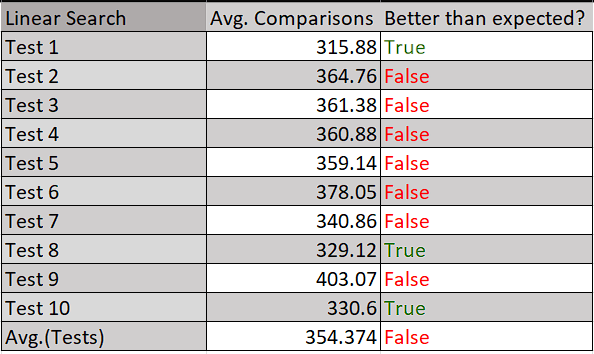
\includegraphics[width=120mm,scale=0.5]{LinSearch.png}
\end{center}
This table diagrams the average time each test took to find all 42 keys in magic items. 
It also depicts how efficient the algorithm was.
Before we continue, it is important clarify a few prerequisites.
\begin{center}
   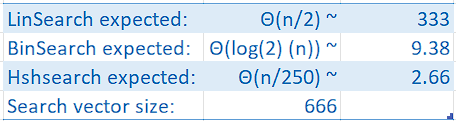
\includegraphics[width=120mm,scale=0.5]{Prerequisites.png}
\end{center}
With these in mind, the "Better than expected?" column now has a basis to compare to.
So over the performed tests, the data shows that only 30\% of all searches for the 42 keys performed were more efficient than the expected value.
Not an amazing look for my code, however only 10 tests were performed, who's to say that if 100 tests took place it wouldn't spread to 50\%?

A binary search was the next task to conquer.
This search takes a key and the middle value of the sorted magic items.
Compares if the middle item is or is not the key, if it is not, then it compares if the middle item is larger or smaller than the key.
Finally if the key is larger than the middle item, the search is ran again on the half greater than the middle.
Otherwise the key is smaller and the search is ran on the half smaller than the key.
\begin{center}
   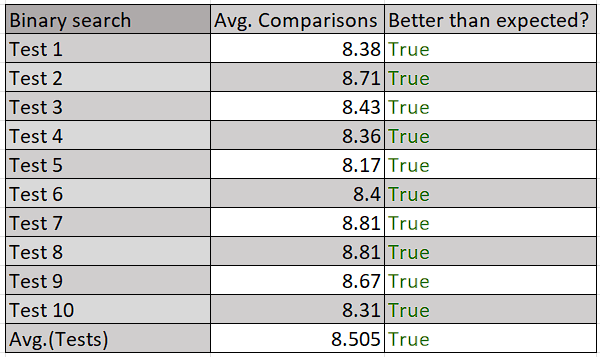
\includegraphics[width=120mm,scale=0.5]{BinSearch.png}
\end{center}
The same 10 tests were performed for binary search with each test's keys being the same for each numbered test.
Meaning, the keys used for test one in linear search were the same keys used for binary search (and for hash searching).
As shown above, the binary searching algorithm I implemented was quite efficient.
But the same logic applied to linear search applies here, although 100\% of tests were more efficient than the average case, does not mean that with more testing it can't be inefficient.

The last search assigned was to take the magic items, create a hash table of 250 buckets, populate it with the items, and search for the keys using the hash table.



\section{Prerequisites} \label{Prereq}


% BREAK DOWN CODE DOC BY DOC FUNC BY FUNC, DON'T WORD FOR WORD, INSTEAD SAY WHAT IT DOES, HOW, WHY, EFFICIENCY...
From Assignment 01 I was able to use my own code to load magic items into a vector and sort it, which saved me time. 




\section{Insertion Sort} \label{Insertion}
The second sorting method was Insertion sort which takes the list and compares each element one by one. 
Meaning the first element is compared to the second, if its greater than the second, swap, then go to the third element, if its less 
than the second swap, if its less than the first, swap again. This continues until the array is sorted
\lstinputlisting[language=C++, firstline=13, lastline=26]{shuffleItems.h}
Record	your	results	in	a	table	in	a	LaTeX	document	along	with	your	
code	listings	and	documentation.	Note	the	asymptotic	running	time	
of	each	search	and	explain	why	it	is	that	way.


Add	these	results	to	your	LaTeX	document,	including	the	asymptotic	
running	time	of	hashing	with	chaining	and	explain	why	it	is	that	
way.

\section{Final Thoughts} \label{Final}
text
\end{document}
